\documentclass[a4paper,11pt]{report}
\pdfoutput=1

\usepackage[english,swedish]{babel}
\usepackage[T1]{fontenc}
\usepackage[utf8x]{inputenc}
\usepackage{listings, babel}
\usepackage{graphicx}
\usepackage[colorlinks=true,linktoc=page]{hyperref}
\usepackage[nonumberlist]{glossaries}
\usepackage{subcaption}
\lstset{breaklines=true,basicstyle=\ttfamily}
\usepackage[margin=2cm]{geometry}
\usepackage{lipsum}

\selectlanguage{english}


\newcommand{\image}[4]{
  \begin{figure}[here]
  \centering
  \includegraphics[width=10cm]{images/#1} 
  \caption[#3]{#4}
  \label{fig:#2}
  \end{figure}
}


\title{Fault detection in photovoltaic systems}
\author{David Nilsson, davnils@kth.se}

\newglossaryentry{MPP}
{
  name=MPP,
  description={maximum power point corresponding to an optimal load}
}

\newglossaryentry{MPPT}
{
  name=MPPT,
  description={maximum power point tracking}
}

\newglossaryentry{solar-module}
{
  name=solar module,
  description={An enclosed box containing several interconnected solar cells}
}

\newglossaryentry{iv-curve}
{
  name=I-V curve,
  description={Plot of panel current as a function of panel voltage}
}


\makeglossaries
\glsaddall

\begin{document}
\pagenumbering{gobble}
\maketitle
\newenvironment{abstractpage}
  {\cleardoublepage\vspace*{\fill}\thispagestyle{empty}}
  {\vfill\cleardoublepage}
\newenvironment{polyAbstract}[1]
  {\bigskip\selectlanguage{#1}%
   \begin{center}\bfseries\abstractname\end{center}}
  {\par\bigskip}

\begin{abstractpage}
\begin{polyAbstract}{english}
This master's thesis concerns three different areas in the field of fault detection in PV systems.
Previous studies have concerned homogeneous systems with a large set of parameters being observed, while this study is focused on a more restrictive case.
The first problem is to discover immediate faults occuring in solar panels.
A new online algorithm is developed based on similarity measures within a single installation.
It performs reliably and is able to detect all significant faults over a certain threshold.
The second problem concerns measuring degradation over time.
A modifed approach is taken based on repetitive conditions, and performs well given certain assumptions.
Finally the third problem is to differentiate solar panel faults from partial shading.
Here a clustering algorithm DBSCAN is applied on data in order to locate clusters of faults in the solar plane, demonstrating good performance in certain situations.

\end{polyAbstract}

\begin{polyAbstract}{swedish}
Det här är en uppsats på master-nivå inom fältet feldetektering av fotovoltaiska system.
Tidigare studier har fokuserat på homogena system med en större mängd observerade parametrar, vilket generaliseras i den här studien.
Den första delen är feldetektering av snabba felförlopp i solpaneler.
En ny algoritm presenteras baserad på grader av likhet inom en enskild solpanelsinstallation.
Den presterar väl och är kapabel att hitta alla singifikanta fel över en viss nivå.
Den andra delen består av att mäta degradering av solpaneler över tid.
En variant av tidigare resultat presenteras som baseras på upprepande förhållanden, vilket presterar väl givet vissa antaganden.
Slutligen hanteras detektering av partiell skuggning och urskiljning av detta från riktiga panelfel.
Lösning är en algoritm DBSCAN som hittar kluster av data i solplanet och den påvisar god prestanda i vissa situationer.

\end{polyAbstract}
\end{abstractpage}

\selectlanguage{english}


\tableofcontents

\chapter*{Preface}
\addcontentsline{toc}{chapter}{Preface}
TBD

\printglossaries
\cleardoublepage
\addcontentsline{toc}{chapter}{\listfigurename}
\listoffigures
\clearpage
\pagenumbering{arabic}

\chapter{Introduction}
TBD

\section{Overview of fault detection}
TBD

\section{Intended readers}
The main target audience interested in this thesis are companies building products in the field of PV power electronics.
Fault detection in solar panels is an active research area and continually evolves, demonstrating an academic interest as well.
The main party interested in the results is of course the supervising company, whom are likely to
integrate a functional solution into their final product.
While being a fairly specialized thesis, it should be comprehensible to anyone with a basic background in statistics.

\section{Scope of this thesis}
The most important scope limitation is that systems should only be studied passively, i.e. the available measurements are used to detect faulty panels.  
Some technical constraints are present as well:
\begin{itemize}
\item The solar panels have 60 or 72 cells built of mono- or poly-crystalline silicon

\item The installations have 14 to 24 panels connected within a small geographic area

\item The available measurements (from each panel) are:
$U$ \footnote{Panel voltage at an optimal load},
$I$ \footnote{Panel current at an optimal load} and
$T_{module}$ \footnote{Low resolution temperature measurement from within the PV inverter}.

\end{itemize}

%TODO: mention that classification of the error is outside the scope

This reflects the consumer market of smaller panel installations with some of the most common panel types.
The type of solar panels constrains the possible output power range and defines appropriate parameters for testing.
Due to time constraints, the simulation of solar panels will largely be based on existing data streams.
These will be used a basis of generating approximate individual panel curves, limiting the amount of effort required.

The supervising provide data feeds providing real time measurements of several PV installations in Sweden.
This data is accumulated in a central database and can be analyzed.
This data has been used in order to verify real-life performance of the classification system, primarily to verify that working systems are not classified as faulty.

Additionally there are other sources that can be used to build realistic simulation models, such as measured solar energy over several years.

\section{Ethical considerations}
TBD
% this section could possibly be integrated into the overview section
% it should deal with sustainability, and argue for why the results of this thesis have a direct impact (with proper sources)
% also have an estimate of how large the improvements can be (probably like a range)
%include: safety hazards (demonstrated), efficiency concerns (demonstrated), reduced work force

\chapter{Background}
This chapter introduces the concept of solar cells, including the underlying physics,
and how they work together with power inverters on the system level.
It is important to have an understanding of the underlying concepts when discussing the applicability of different methods to failure detection.
These concepts are however generic and common knowledge in the field of PV power generation, 
hence this chapter can be skipped given a sufficient existing background.

\section{Theory of the solar cell}
Solar cell technology can be broadly described as equipment converting incoming photons (typically sunlight) to electric energy.
The solar cells of interest in this study are mono- and poly-crystalline Silicon, technologies that currently have a large market share\cite{Zhao2010thesis}.

Both of these share the property of being being constructed around a single pn-junction, i.e. the connection between two differently doped Silicon areas.
The incoming photons may be absorbed by the Silicon in which case a electron-hole pair is created\cite{Zhao2010thesis}, since the electron is pushed to an outer layer by the absorbed energy.
Connecting an electric load, such as a heating element, to the terminals of the solar cell will then induce a DC current.
Overall this results in an efficiency of $13-18\%$ for single-junction Silicon technology\cite{Zhao2010thesis}.

The solar cell can by analyzed by building an equivalent electrical circuit from well-defined components.
A broadly used model is the one-diode model\cite{Walker2001} as shown in figure \ref{fig:solar-cell-equiv}.
It is based on modelling the solar cell as a current source connected in parallel with a diode.
In addition there are inherent losses due to imperfect manufacturing.
These are modelled as a series and a parallel resistance.
The resulting current $I_{load}$ flows across the terminals through a load with potential difference $U_{load}$.
$I_{photo}$ corresponds to the amount of current generated by incoming photons which is proportional to the irradiance and area of the solar cell.

\begin{figure}[!ht]
\centering
\begin{subfigure}{0.4\textwidth}
  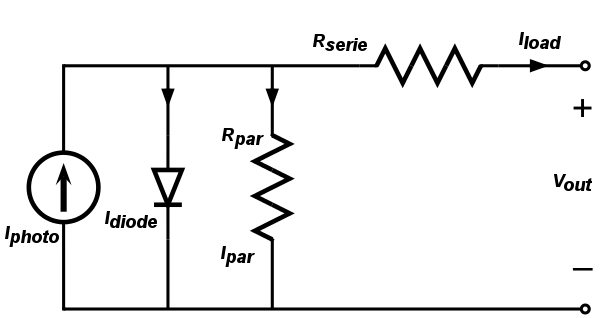
\includegraphics[width=\linewidth]{solar-cell-equiv.png}
  \caption[Equivalent circuit of a solar cell]{
    Equivalent circuit of a solar cell based on a current source and diode,
    with losses represented by a series and a parallel resistance.
  }
  \label{fig:solar-cell-equiv}
\end{subfigure}
~
\begin{subfigure}{0.4\textwidth}
  \begin{tabular}[b]{| c | c |}
  \hline
  $I_{load}$ & load current \\ \hline
  $U_{load}$ & load voltage\\ \hline
  $I_{photo}$ & photogenerated current \\ \hline
  $I_{diode}$ & diode current \\ \hline
  $I_{par}$ & parallel loss current \\ \hline
  $R_{par}$ & parallel loss resistance \\ \hline
  $R_{serie}$ & series loss resistance \\ \hline
  \end{tabular}
  \caption[solar-cell-variables]{Variables of the one-diode model.}
  \label{fig:one-diode-model-vars}
\end{subfigure}
\end{figure}

The model can be formalized in order to solve for the resulting current and voltage, given the parameters of a solar cell.
Summing up all the currents it holds that $I_{photo} = I_{diode} + I_{par} + I_{load}$.
Using the well known Ohm's law followed by Schokley's diode equation\cite{Walker2001}, the following holds:

\begin{multline}
\label{eq:eq-circuit}
I_{load} = \\
I_{photo} - I_{diode} - I_{par} = \\
I_{photo} - I_{diode} - \frac{R_{serie}I_{load} + U_{load}}{R_{par}} = \\
I_{photo} - I_{sat}(e^\frac{q(R_{serie}I_{load} + U_{load})}{k_B T} - 1) - \frac{R_{serie}I_{load} + U_{load}}{R_{par}}
\end{multline}

$I_{sat}$ denotes the constant saturation current of the diode,
$k_B \approx \SI{1.38e-23}{\joule\per\kelvin}$,
and $q \approx \SI{1.60e-9}{\coulomb}$.

The free variables are $I_{load}$, $U_{load}$ and $T$, where $T$ is the temperature measured at the p-n junction.
All parameters of the model, such as $I_{sat}$, may be given in a datasheet or can alternatively be extracted by performing non-linear regression based on samples of the free variables\cite{Walker2001}.

There are several relevant aspects in understanding this equivalent model when performing analysis of power generated from solar panels.
Firstly the output current is proportional to the incoming irradiance, which directly affects $I_{photo}$.
Figure $\ref{fig:trina-iv-curve}$ shows a plot of $I_{load}$ as a function of $U_{load}$ at different irradiations.
The panel is held at a constant temperature.

%TODO: Mention that this is actually several cells connected in series.. still reflects the behaviour of a single cell
\image{trina-60cell-iv-alpha.png}{trina-iv-curve}{Trina P05 IV-curve characteristic}{
  TBD
}

In addition to changing irradiation there might also be a range of operating temperatures depending on local weather conditions.
The temperature affects the second term in equation \ref{eq:eq-circuit} and increased temperature results in decreased load current.
This is important to take into account since otherwise increased temperature might be mistaken for decreased irradiation.
While being an important source of measurements in general, this study only concerns fault detection based on samples of $I_{load}$ and $U_{load}$, but still needs to perform reliable classification.

Finally, it is important to realise that different solar panels have different parameters and will yield different I-V curves.
This implies that inhomogeneous systems offer challenges when comparing produced power output, for example in the case of fault detection.

\section{Systems of solar panels}
The solar cells described previously typically generate an output voltage of at most a few volts\cite{Zhao2010thesis}.
A solar module connects several solar cells and places them into a rigid enclosure.
This module can then be mounted as part of a larger system.
Figure \ref{fig:solar-module-generic} shows a 54-cell module with the output DC terminals visible on the backside.

%TODO: Add a schematic
\image{solar-module-generic.jpg}{solar-module-generic}{Generic solar module}{
  Back and front of a generic 54-cell Silicon solar module. Every cell and the vertical interconnections are clearly visible.
}

In addition to protecting the fragile Silicon sheets, the purpose of the module is also an to contain the photons by using a anti-reflective coating.
This thesis considers modules containing 60 or 72 solar cells of the previously specified type, connected in series.
The resulting I-V curve of the module has an increased width and every point is stretched to $n \cdot U_{load}$ with $n$ cells each producing at some $U_{load}$.

There is however also some extra components involved in the module circuitry.
Figure \ref{} shows a schematic of a xx-cell module.

The panel is divided into y substrings of which each has a diode connected in parallel.
During normal operation the diodes will not carry any current.
If some cell is reduced in performance, for example by having an unusually high series resistance, this will result in the corresponding diode conducting the current, effectively bypassing that specific substring\cite{Roman2006}.
This is relevant since the I-V curve will reflect these properties and should be analyzed while keeping these effects in mind.

\section{The role of PV inverters}
Solar panels produce DC current as previously described.
This is suitable for certain types of applications such as charging batteries.
It is however not suitable for generation on the electric grid which uses AC power at a fixed voltage.
This translation is done using a power inverter, also known as PV inverters.
There are different topologies applicable, i.e. different arrangements of both solar panels and PV inverters.
Traditionally a common configuration has been to use long strings of modules connected in series with a single big inverter at the end of the string.
This approach is however constrained due to individual modules having an unproportional influence on the total power yield of the string \cite{Roman2006}.

\image{optistring-inverter.jpg}{optistring-inverter}{Optistring PV inverter}{
  The distributed Optistring PV inverter with DC input and AC output.
  A separate inverter is placed on the back of every solar panel.
}

The system considered in this study is a distributed version with a typical inverter shown in figure \ref{fig:optistring-inverter}.
Each module has its own simple PV inverter acting as an independent AC power source.
In addition to providing higher efficiency, this also produces $I_{load}$ and $U_{load}$ measurements from every individual module.
This is highly relevant since studies in fault detection typically consider a specific topology and the results might not always generalize to the distributed case.

A PV inverter should transform the power in the most efficient way and more specifically ensure that the panel is being applied to an optimal load.
This corresponds to finding the point on the I-V curve where $I_{load} \cdot U_{load}$ is maximal.
The maximum point is known as MPP and is typically found using some kind of search method along the I-V curve.
Examples of this includes Pertube and Observe and Incremental conductance\cite{Roman2006}.
These are relevant to this study since local searches may not be well-behaved during panel faults\cite{Roman2006}.
This is due to the existence of multiple local maxima on the I-V curve, resulting in the possible of considering a local optima as a global maxima.
Previous studies have also found that MPP tracking, known as MPPT, might prevent faults from being observed during night-to-day transitions\cite{Zhao2010night}.

A relevant term applicable to measuring the efficiency of solar cells is \emph{fill factor} which is defined as the ratio between the power at $I_{MPP} \cdot U_{MPP}$ and $I_{max} \cdot U_{max}$.
The maximum reference values are defined as $I_{max}$ being the current measured in closed circuit and $U_{max}$ being the voltage measured without any load connected.


\section{Solar power in practice}
Given an understanding of the different components of a PV solar installation it is also important to reflect on real-life behaviour.
The power output of an installation and individual solar panels vary to a large degree.
Figure \ref{fig:january-power-curve} and \ref{fig:october-power-curve} illustrate this, where a 10-fold decrease in peak power output is seen over a period of 3 months.
In addition the total duration of power output is reduced by 4 hours.
Another interesting aspect of these graphs is the significant amount of noise present due to shadowing.

\begin{figure}[here]
\centering
\subimage{january-power-curve.png}{january-power-curve}{TBD}{
  Power curve (in Watt) captured from a 16-module installation based in Stockholm, Sweden, captured in the month of January 2014.
}{0.48}
~
\subimage{october-power-curve.png}{october-power-curve}{TBD}{
  Same system as in figure \ref{fig:january-power-curve} captured in October 2013.
}{0.48}
\end{figure}

After sunset and during periods of negligible irradiance the system is completely shutdown in order to increase efficiency.
In addition to seasonal and geographical dependencies, the power output is also proportional to the number of solar panels in the system and the type of each panel.
All of these highly varying conditions impose restrictions on how fault detection can be implemented and the required scope of validation.
The main point is that developed methods need to be dynamic and adaptive to any applicable system configuration.

\chapter{Theory of fault detection}
Based on knowledge of how a PV system produces energy and the underlying dependencies,
it is possible to reason about faults.
Faults in PV systems can be characterized as permanent power losses but a more fine-grained analysis might be suitable if there are failure-specific patterns that can be utilized.
This chapter gives an overview of possible failure conditions and describes the different kinds of methods that have been established by previous studies.

% mention OCPD, GPD, and possible other types of existing protection devices
% also bind these to the insufficient protection (as shown by the thesis and others)
% provides a great motivation: both environmental and safety improvements through this work.

\section{Issues in photovoltaic systems}
several issues present in PV systems \cite{Baltus1997,King2002,Petrone2008}.

list of errors \cite{Stettler2005}

One study \cite{Munoz2011} discusses the following failures in solar modules:
\begin{itemize}
\item Yellowing and browning
\item Delamination
\item Bubbles in the TODO
\item Cracks in cells
\item Defects in anti-reflective coating
\item Hot spots caused by TODO
\end{itemize}

Another study\cite{Forman1982} identified the following conditions:
\begin{itemize}
\item Edge-seal delamination
\item Newly cracked cells
\item Delamination over cells and interconnections
\item Split encapsulation over cells and interconnections
\item Protruding interconnections
\end{itemize}

It has also been found that connections and the weldings connectors can be degraded over time \cite{Houssein2010}.

In conclusion it can be said that there is a wide range of failure conditions and TODO.
This breadth motivates the use of classes of failures, such as the TODO used by TODO. 

\cite{Zhao2010thesis} and the following papers \cite{Zhao2012tree,Zhao2013graph,Zhao2013outlier} uses a categorization (ground, line-line)
mention that classification is out of scope for this thesis.

dust is a problem \cite{Mani2010} at certain geographical locations

early degradation occurs \cite{Munoz2011}, tie to warranty

\section{Partial shading of solar panels}
TBD

(partial) shading is seen as an error \cite{Stettler2005} %verify citation

study with plots \cite{Alsayid2013} 

study with applicable method \cite{Firth2010}

"the proposed algorithm can differentiate easily whether it operates under the temporary partial shading..." \cite{Kang2012}

percentual rates of degradation \cite{Quintana2002}

\section{Approaches to fault detection}
TBD

%discuss limitations and applicability of individual papers
comparison with a known reference (based on satellite data) \cite{Stettler2005}
analytical model \cite{Chouder2010}, \cite{Raina2013}, \cite{Chao2008}, parameter extraction \cite{Eicker2005}, \cite{Chouder2009} and \cite{Walker2001}
analysis of IV-curves and short circuit currents \cite{Meyer2004}
inferential statistics \cite{Vergura2008,Vergura2009}
graph-based \cite{Zhao2013graph}
decision tree \cite{Zhao2012tree}
outlier detection \cite{Zhao2013outlier}
kalman \cite{Kang2012}

locating faults within an array of panels \cite{Lin2012}

\section{Measuring degradation}
TBD

IR-based camera snapshots, "EL image technique", "I–V curve analysis can be performed string by string" \cite{Munoz2011}
degradation seen as losses present over long time periods \cite{Stettler2005}

master's thesis discusses classification of degradation, seen as additional series resistance \cite{Zhao2010thesis}
performs verification of the implemented methods by adding resistance over time (potentiometer)

degradation effect on fill-factor \cite{Raina2013}

least-squares on lots of data, annual comparisons \cite{Makrides2010}


%TODO: Aren't there any automatic methods? pretty sure that degradation has shown up as a classification category <- !
%      This should be explicitly mentioned. The master's thesis lists degradation as a condition producing a current decrease.


\chapter{Analysis}
TBD


\chapter{Results}
TBD

\section{Conclusion}
TBD

\bibliographystyle{abbrv}
\bibliography{../ref.bib}

\end{document}
